\chapter{Methodology}
define  features that I will use for classification how I decided on this and motivation behind these features.

\section{Characteristics of Japanese}
talk about about Japanese text is processed in regards to how it will be treated for my analysis
   Kanji vs. Hiragana, - since dealing with learner texts, the lower learners have a preference for hiragana so this
is taken into consideration when matching grammatical forms. - for the most part the tokenizer seems to be able to
still parse when using only hiragana - but of course spelling errors can through this off.

What is considered a word in Japanese may differ from other languages. In English, a bound morpheme may be treated as an individual word; however, this is not the case in Japanese. For example, the word 話す\textit{hanasu}(to speak) would be considered one word, but the potential form 話せる \textit{hanaseru}(to be able to speak) would be considered two separate words consisting of \textit{hanas} and \textit{eru}.

\section{About corpus}
information about the IJATS corpus organization, prepossessing,

This study utilizes data from the International Corpus of Japanese as a Second Language (I-JAS), as detailed in \citet{Sakoda2020}.  The I-JAS corpus includes both spoken and written samples of Japanese from a diverse pool of 1,000 adult learners aged between 17 and 63 years, all of whom are learning Japanese as a second language. Native speaker samples are also included in the corpus.

To assess each participant's proficiency level, the Japanese Computer Adaptive Test (J-Cat) by \citet{Imai2009} was administered. Further information about this test, including its scoring methodology, is provided in the subsequent section. In addition to language proficiency data, various metadata, such as participants' native language, prior experiences of visiting or living in Japan, and current location (whether outside or within Japan), were also recorded.

From the larger pool of participants, writing samples were obtained from 687 individuals, including a control group of 48 native speakers. A breakdown of the proficiency groups among these 687 participants who submitted writing samples is presented in Table 1.

%need to update this table to account for JLPT levels, N5, N4, N3, N2, N1
\begin{table}
\centering
\begin{tabular}{lrl}
\hline \textbf{Proficiency Level} & \textbf{\# of Participants} \\ \hline
Basic & 15 \\
Pre-Intermediate & 81 \\
Intermediate & 199\\
Intermediate High & 187 \\
Pre-Advanced & 122 \\
Advanced & 34\\
Native & 48 \\
\hline
\end{tabular}
\caption{\label{participants-chart} breakdown of participants per proficiency level}
\end{table}

\subsection{Writing Tasks}

% add the additional SW 1 and 2 tasks where participants were expected to write a story based on a picture.
Each participant submitted four samples of writing for specific tasks:
\begin{itemize}
    \item A short essay titled "Our Eating Habits," involving a comparison between fast food and home-cooked meals in the learner's home country.
    \item A letter addressed to a former teacher, requesting a letter of recommendation for a scholarship application.
    \item An email seeking an extension for the deadline of a report submission.
    \item An apology email in which the learner must decline an invitation.
\end{itemize}
These tasks were consistent across all participants, regardless of their proficiency levels, and encompassed various task types. The inclusion of a range of task types and formalities was intended to encourage diverse responses from the students and mitigate a potential "task effect" similar to what  was described in \cite{Alexpoulou2017}. The writing samples were processed-as-is without being corrected for learner errors.

\subsection{J-CAT test}
Developed in 2009 since depreciated/discontinued with no new updates to account for new JLPT scoring implemented in 2010
background and information on the J-CAT test compare to JLPT


The J-Cat, short for Japanese Computerized Adaptive Test \cite{Imai2009}, is a computer-administered assessment that
evaluates an
individual's proficiency in the Japanese language. Although it has been depreciated, Japanese universities widely
employed this test as an efficient tool for assessing the language skills of foreign students seeking placement in
Japanese language courses. This adaptive examination tailors its question difficulty to a student's performance in
the areas of Vocabulary, Grammar, Listening, and Reading. At the time of its' release the test related its scores in
terms of the JLPT levels

\begin{figure}[h]
    \centering
    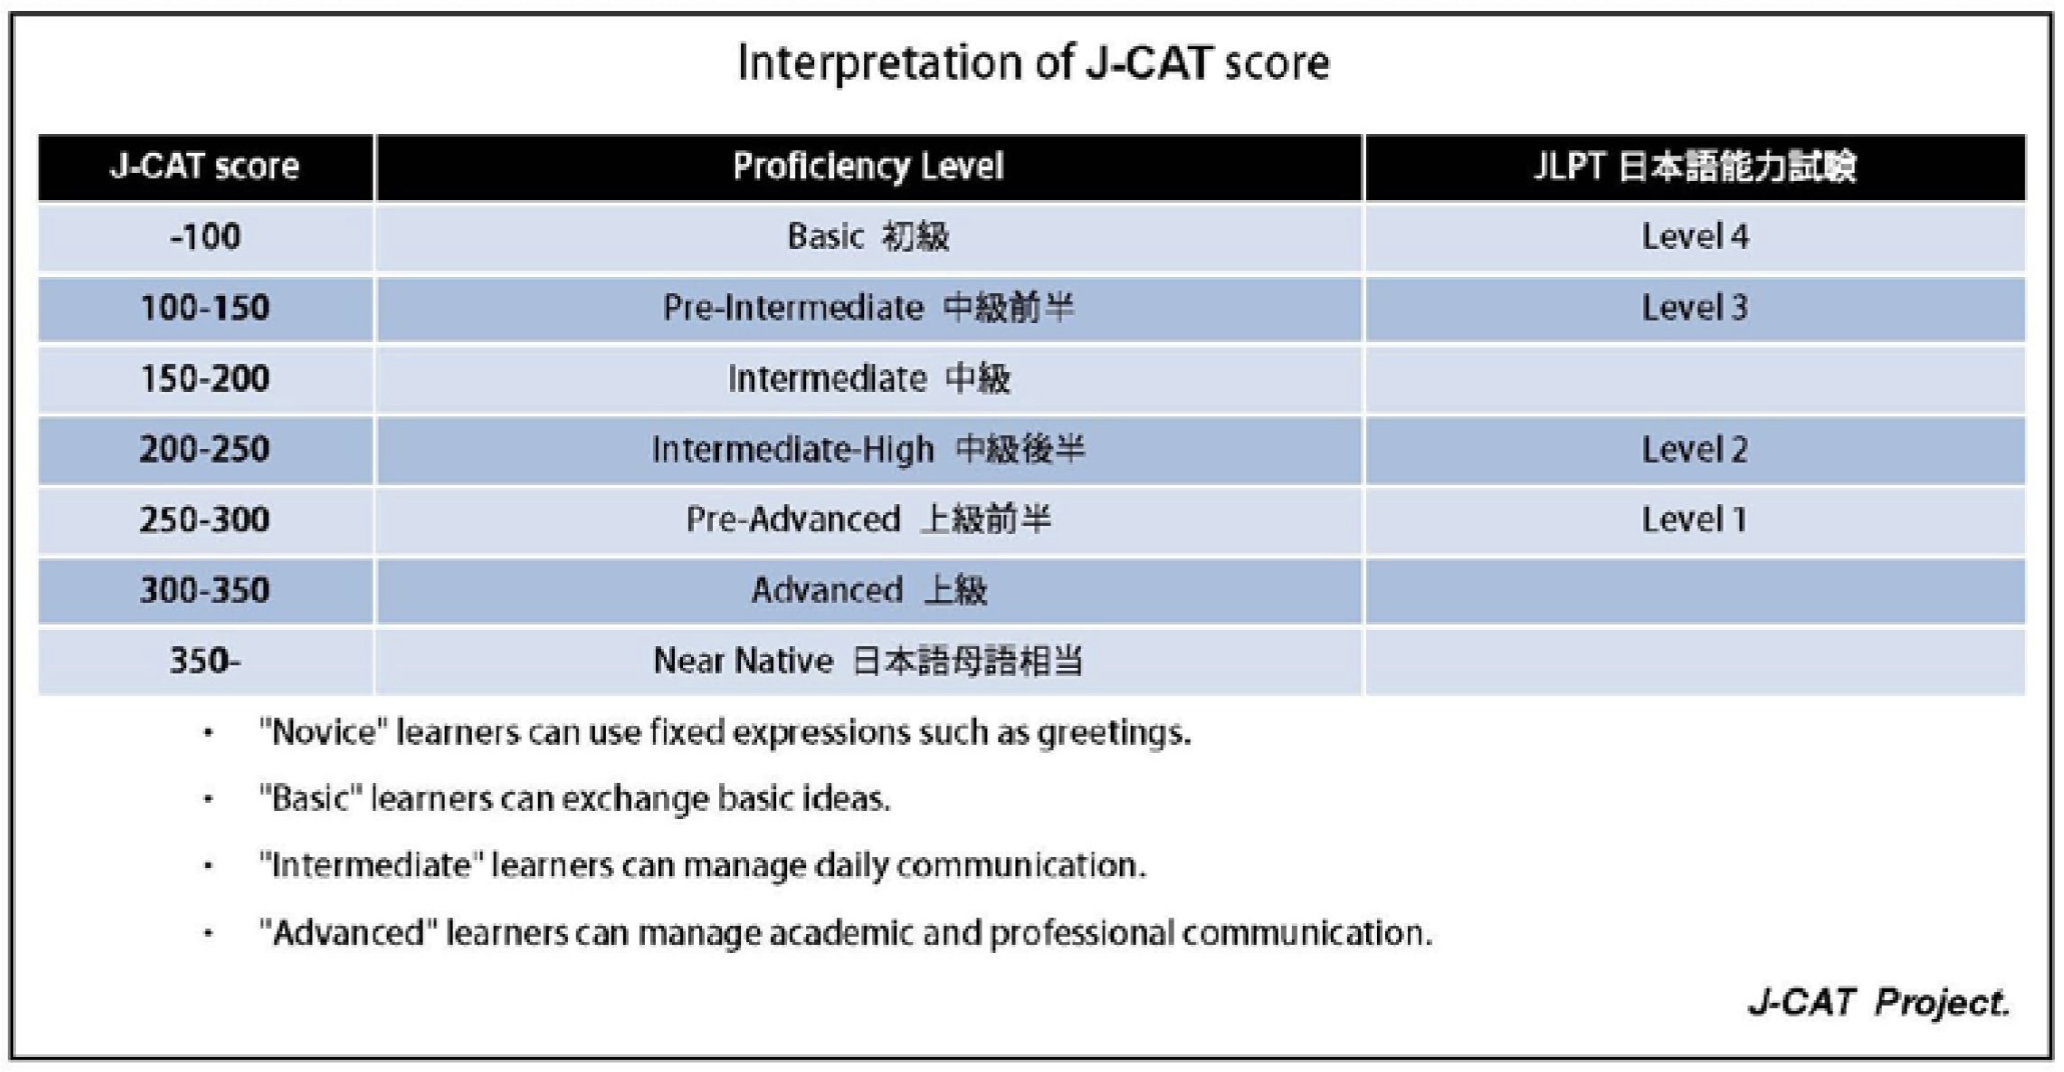
\includegraphics[scale=.3]{img/JCatScores.png}
    \caption{The assigned proficency levels from the J-Cat test as taken from the original paper}
    \label{fig:JCatLevels}
\end{figure}

Each student receives a numerical score that corresponds to one of seven distinct proficiency levels, as detailed in
Table \ref{tab:proficency-table}. This study will categorize participants according to their J-Cat proficiency level. Participants in the
native speaker control group were given a default J-cat score of 999.

\begin{table}
\centering
\begin{tabular}{lrl}
\hline \textbf{Proficiency Level} & \textbf{J-Cat Score}  \\ \hline
(N5) Basic & 0-100 \\
(N4) Pre-Intermediate & 100-150 \\
(N3) Intermediate & 150-200 \\
(N2) Intermediate-High & 200-250 \\
(N1) Pre-Advanced & 250-300 \\
Advanced & 300 - 350 \\
Near Native & 350+\\
\hline
\end{tabular}
\caption{\label{tab:proficency-table} Proficiency level classification based on J-cat score. The JLPT equivalent of the score is given in parenthesis.}
\end{table}


\section{Complexity Measures}
detail the complexity measures I will use, how I developed the scripts to automatically "extract them" and the statistical significance between the proficiency levels
list, Sent Length, Clauses per sentence, Noun phrase length,  Subordination, coordination, noun phrase length, MTLD,Morphological complexity? , ADD measures?

\section{Criterial Features}
Describe the rule based feature matcher I made for extracting certain grammatic patterns to disconcern their use
across proficentcy levels. Mention how many grammar points at each level I was able to include. Use of the lower
levels doesn't disconcern much so focus should be on the intermediate and upper levels.  Forms that are mainly form
based(and therefore easier to pattern match) should be given priority over. Give some examples of rules derrived

mention that I chose forms which spanned multiple levels. I.e. しか at N4 used with Nouns and しか〜ないat N3 used
with verbs to see if their use at the different levels actually follows this.

don't forget about implementing normallization.

\section{EBMS}
 Here I will give a breif overview of Explainable boosting machines and why I chose them for my analysis.


% Give up on this part

%\section{Criterial Features}

%\section{Automatic Error Annotation}

%Explain how I will do this so that I will further be able to extract criterial features to examine
% - Automated Error Detection?
%    can I apply an LLM to check each sentence, and then use distance measure to classify errors
%    -what about discourse errors? I have a feeling these will not be caught by an LLM...
%        disregard discourse errors.
%    need some way to measure errors when the corpus is uncorrected.

%    measure correct or incorrect particles?
%    can I train a classifier for automatic error annotation for particles?
%        using SNOW-NLP/snow_simplified_japanese_corpus for training?
%        格助詞 - が, の, を, に, へ, と , で, から, より
%        係助詞 - は, も, こぞ, でも, しか, さえ, だに
% - Which type of errors will I annotate for?
%        - Automated detection of particle errors - using work?